\documentclass[UTF8]{ctexart}
\usepackage{amsmath}
\usepackage{geometry}
\usepackage{graphicx}
\usepackage{gensymb}
\usepackage{wrapfig}
\usepackage{titlesec}
\usepackage{float}
\geometry{a4paper,scale=0.8}
\title{2016年电磁场与波期末试题}
\author{Deschain}
\titlespacing*{\section}
{0pt}{0pt}{0pt}
\titlespacing*{\subsection}
{0pt}{0pt}{0pt}
\titlespacing*{\paragraph}
{0pt}{0pt}{0pt}
\titlespacing*{\subparagraph}
{0pt}{0pt}{0pt}
\begin{document}
\maketitle
\section{}
\begin{wrapfigure}{r}{3cm}
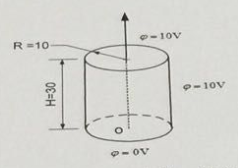
\includegraphics[width=3cm]{2016-1.png}
\end{wrapfigure}
\paragraph{}
一个三维柱型区域静电场边界条件如右图。
\subsection{}
\paragraph{}
求区域内的电位分布$\varphi(\rho,\phi,z)$的解析表达式,通解的选取需要说明理由(10分)。
\subparagraph{解答}
\[\varphi=10+\sum_i^{\infty}{A_iJ_0(k_z\rho)sh(k_z(H-z))}\]
\[i=0,2,4\cdots\]
\subsection{}
\paragraph{}
在答题纸上用虚线画出过Z轴平面内等位线(5分)。
\subsection{}
\paragraph{}
在答题纸上用虚线画出过Z轴平面内电力线(5分)。
\subparagraph{解答}
\begin{figure}[htbp]
\centering
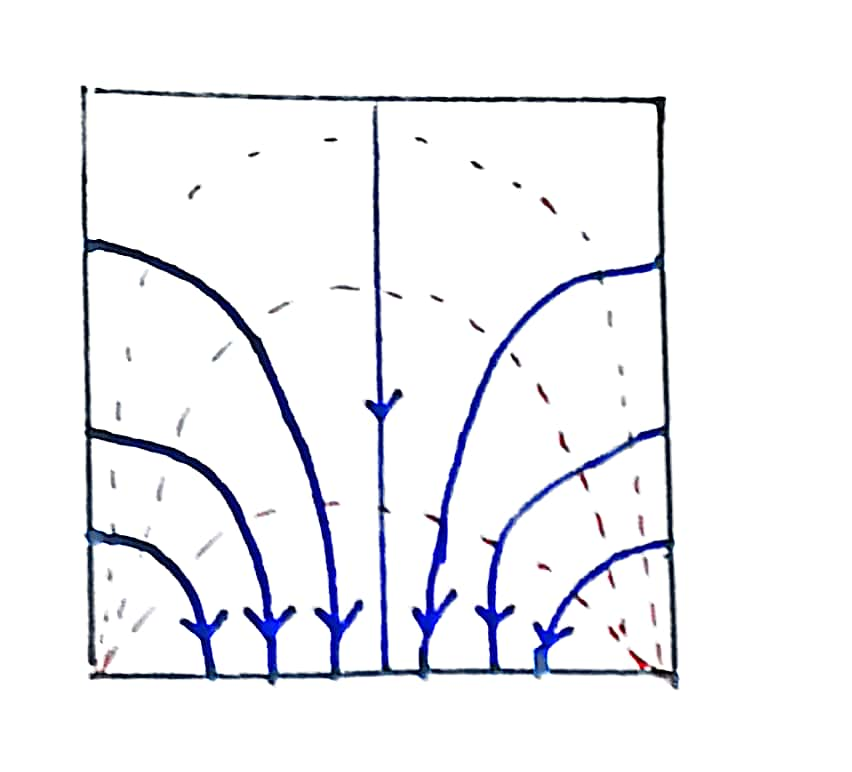
\includegraphics[width=3cm,height=3cm]{2016-2.jpg}
\end{figure}
\subsection{}
\paragraph{}
在0时刻,Z坐标轴上Z=15处有一个静止的带正电荷的球;假设球和边界均为不形变的刚体,不存在重力,仅存在电磁力,碰撞时不损失能量;请文字描述该球在0时候以后的运动轨迹,不需要公式。(5分)
\subparagraph{解答}
从Z=15加速运动到Z=0,碰撞后速度反向,减速运动到Z=15,停下。重复上述过程。
\section{}
\paragraph{}
无限大自由空间中:
\subsection{}
\paragraph{静电场}
有一组电荷分布在坐标系原点附近,且所有电荷均分布在x,y或z轴上。现在需要在x轴上远离坐标原点的所有位置上均产生归一化电场矢量$\frac{\vec E}{\lvert E\rvert}=\frac{\sqrt 2}{2}\hat x+\frac{\sqrt 2}{2}\hat y$,请给出这组电荷中各电荷的坐标、电荷正负、相对电荷量。(10分)
\subparagraph{解答}
+q:(0,-d,0)\\
-q:(0,d,0)\\
+q:(-d,0,0)\\
-q:(d,0,0)
\paragraph{时变电磁场:}
假设辐射源集中在坐标系原点附近,是否可能在x轴上远离坐标原点的所有位置上产生瞬时归一化电场矢量$\frac{\vec E}{\lvert E\rvert}=\frac{\sqrt 2}{2}\hat x+\frac{\sqrt 2}{2}\hat y$?如果可以,请说明产生的方式。如果不可以,请说明原因。(5分)
\subparagraph{解答}
不可能。辐射场没有$\hat r$分量。
\paragraph{时变电磁场:}
假设辐射源在原点,请写出-Y轴上远离坐标原点的归一化幅度为1的右旋圆极化波的电场的完整复数表达式(包括波动项、时谐项)。(5分)
\[\vec E=(\hat x-j\hat z)e^{j(\omega t+ky)}\]
\paragraph{时变电磁场:}
给出两种产生这个圆极化波的具体方法。(5分)
\subparagraph{解答}
[法一]:沿x,z轴正向各放一个等大的电偶极子,x轴上的超前z轴上的$\frac{\pi}{2}$。
[法二]:沿z轴正向放一个电偶极子,在直线${z=0,y=\frac{\lambda}{4}}$上沿x轴正向放一个电偶极子,两者大小相等。
\section{}
由两块位于y=0和y=4的无穷大理想金属板构成的平板波导。一个频率为300MHz电磁波在其中沿+X方向传播。全空间$\epsilon_r=1$;$\mu_r=1$。
\subsection{}
请问d=5mm的时候,电磁波是否可以传播?如果可以,该电磁波是什么波?如果不可以,请给出原因。(5分)
\paragraph{解答:}
可以传播,是TEM波。
\subsection{}
如果希望用该平板波导传300MHz TE波,请问d的最小尺寸是多少?
\begin{equation*}
d \geq \frac{\pi}{k}=0.5m
\end{equation*}
请写出平板波导中TE波基模的所有电场、磁场分量的完整复数表达式(包括波动项、时谐项),实数系数及符号可以合并,虚数符号j的关系必须正确。(5分)
\begin{equation*}
\begin{aligned}
&\vec E=Ajsin(\frac{n\pi}{d}y)e^{j(\omega t-kx)}\\
&\vec H=(Bjsin(\frac{n\pi}{d}y)+Ccos(\frac{n\pi}{d}y))e^{j(\omega t-kx)}
\end{aligned}
\end{equation*}
\subsection{}
画出$[0,\lambda_x]$的TE基模三维电磁场结构(电场用实线,磁场用虚线)。
\begin{figure}[H]
\centering
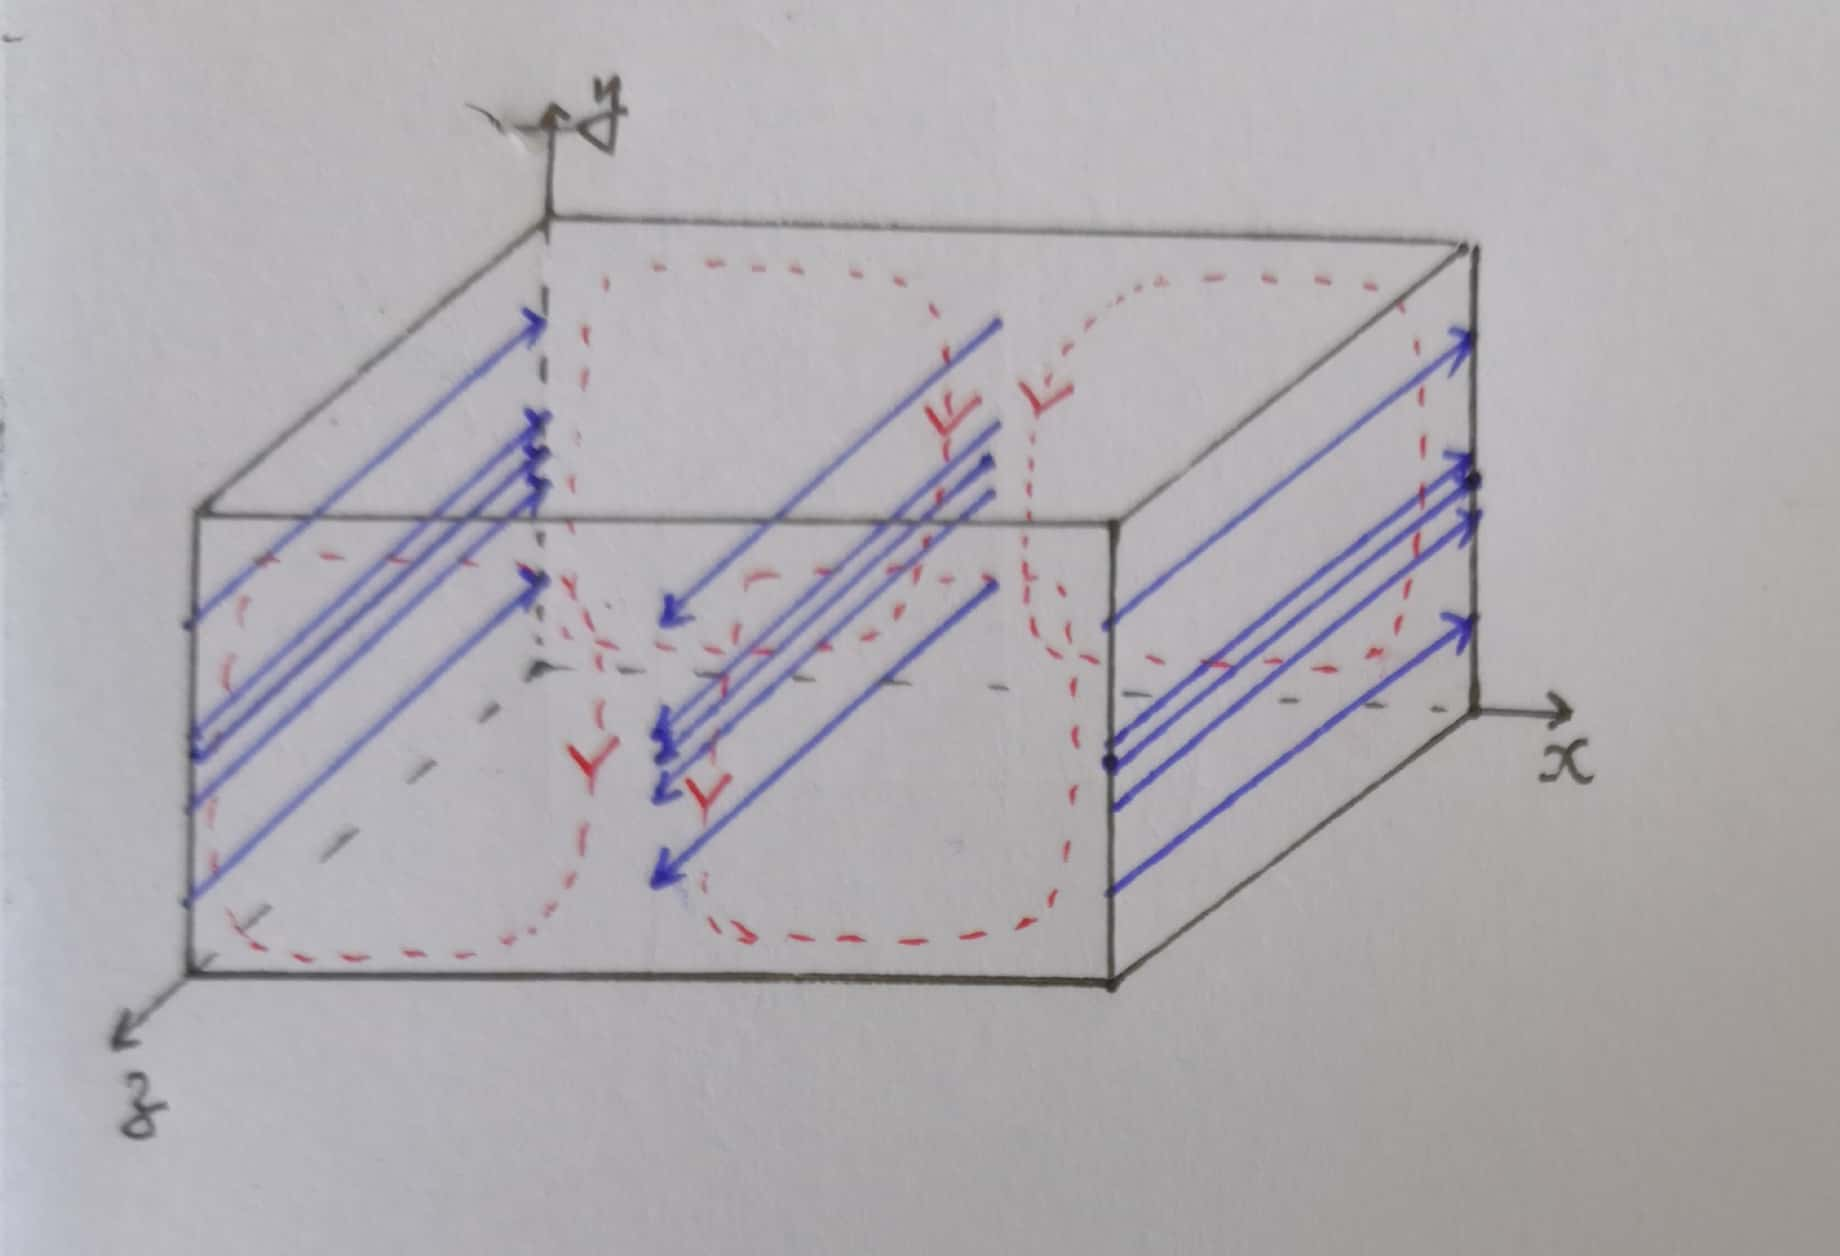
\includegraphics[width=6cm,height=3cm]{2016-3.jpg}
\end{figure}
\subsection{}
画出$[0,\lambda_x]$的TM基模三维电磁场结构(电场用实线,磁场用虚线)。
\begin{figure}[H]
\centering
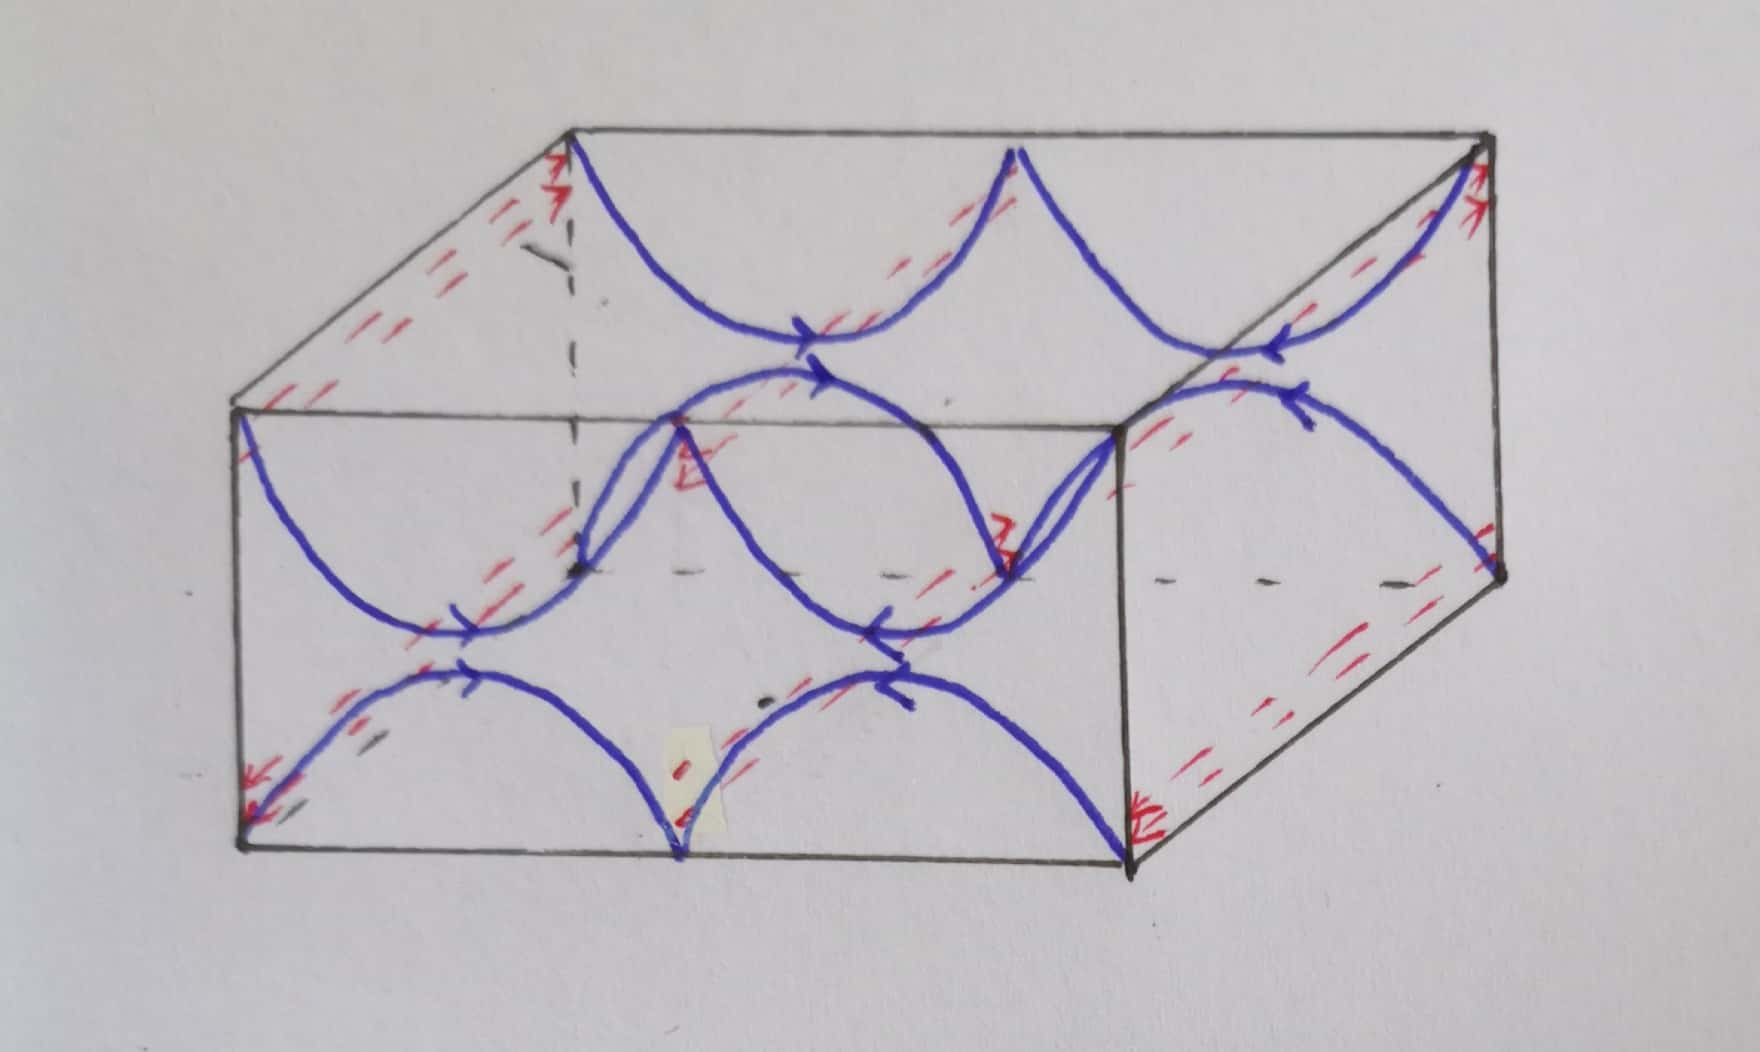
\includegraphics[width=6cm,height=3cm]{2016-4.jpg}
\end{figure}
\section{}
\begin{wrapfigure}{r}{4cm}
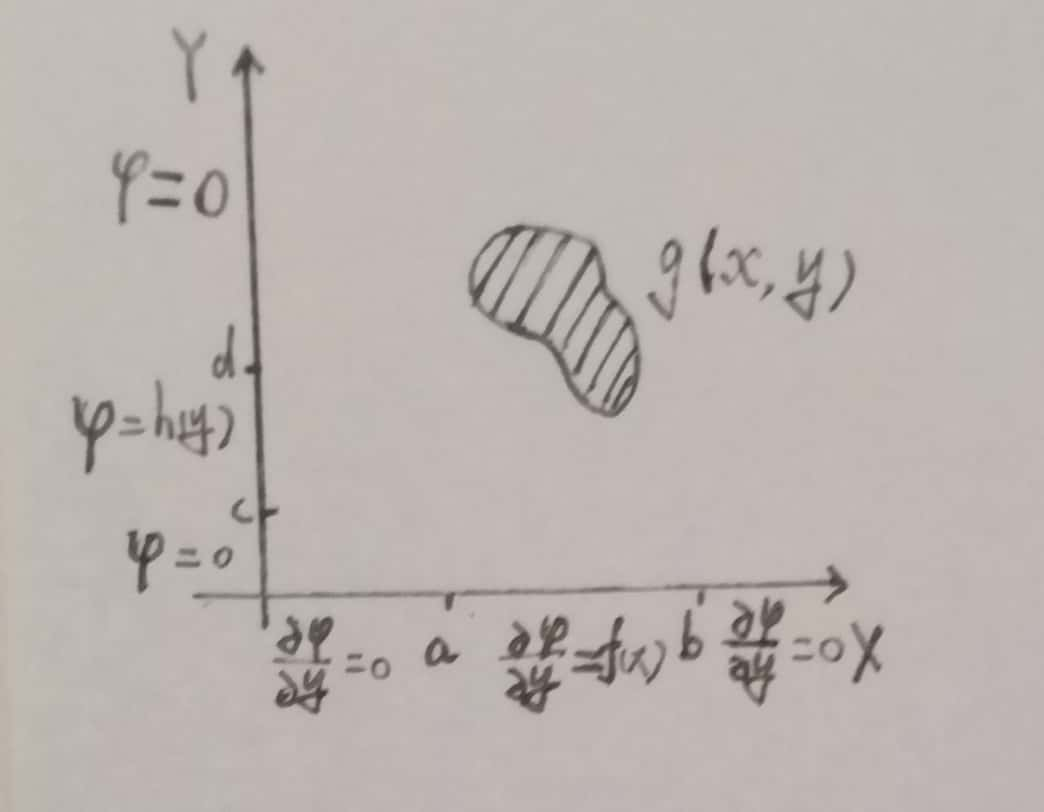
\includegraphics[width=4cm]{2016-5.jpg}
\end{wrapfigure}
右图所示二维静电场问题中,研究的区域为第一象限。X,Y正半轴构成边界。边界上一共存在4类边界条件。图中的灰色区域为电荷分布g(x,y)。
\subsection{}
请给出本问题所对应的格林函数G(x,x',y,y')在空间满足的偏微分方程。(5分)
\[\nabla^2G(\vec r,\vec r')=-\delta(x-x',y-y')\]
\subsection{}
请问这是格林函数的第几类边值问题?请给出该问题格林函数需要满足的边界条件。(5分)
第三类边值问题。边界条件:
\[G\lvert_{x=0}=0,\quad\quad\frac{\partial G}{\partial n}\lvert_{y=0}=0\]
\subsection{}
请利用格林函数计算本问题的积分表达式。$\varphi(\vec r)=$?需要准确给出积分区域、积分起始点。(5分)
\[\int_S^{}{\frac{\rho G}{\varepsilon}dS}-\int_a^b{Gf(x)dx}+\int_c^d{h(y)\frac{\partial G}{\partial x}dy}\]
其中S是g(x,y)存在的区域。
\subsection{}
请给出该格林函数的解析解$G(\vec r,\vec r')$。(提示:二维问题,通解ln)(5分)
\begin{equation*}
\begin{aligned}
&G(\vec r.\vec r')=\frac{1}{2\pi}ln(\frac{r_2r_3}{r_1r_4})\\
&r_1=\sqrt{(x-x')^2+(y-y')^2}\\
&r_2=\sqrt{(x+x')^2+(y-y')^2}\\
&r_3=\sqrt{(x+x')^2+(y+y')^2}\\
&r_4=\sqrt{(x-x')^2+(y+y')^2}
\end{aligned}
\end{equation*}
\subsection{}
假定源点位于(x',y'),在答题纸上(不是试卷)画出该格林函数的电力线(实线)、电场线(虚线)。(5分)
\begin{figure}[H]
\centering
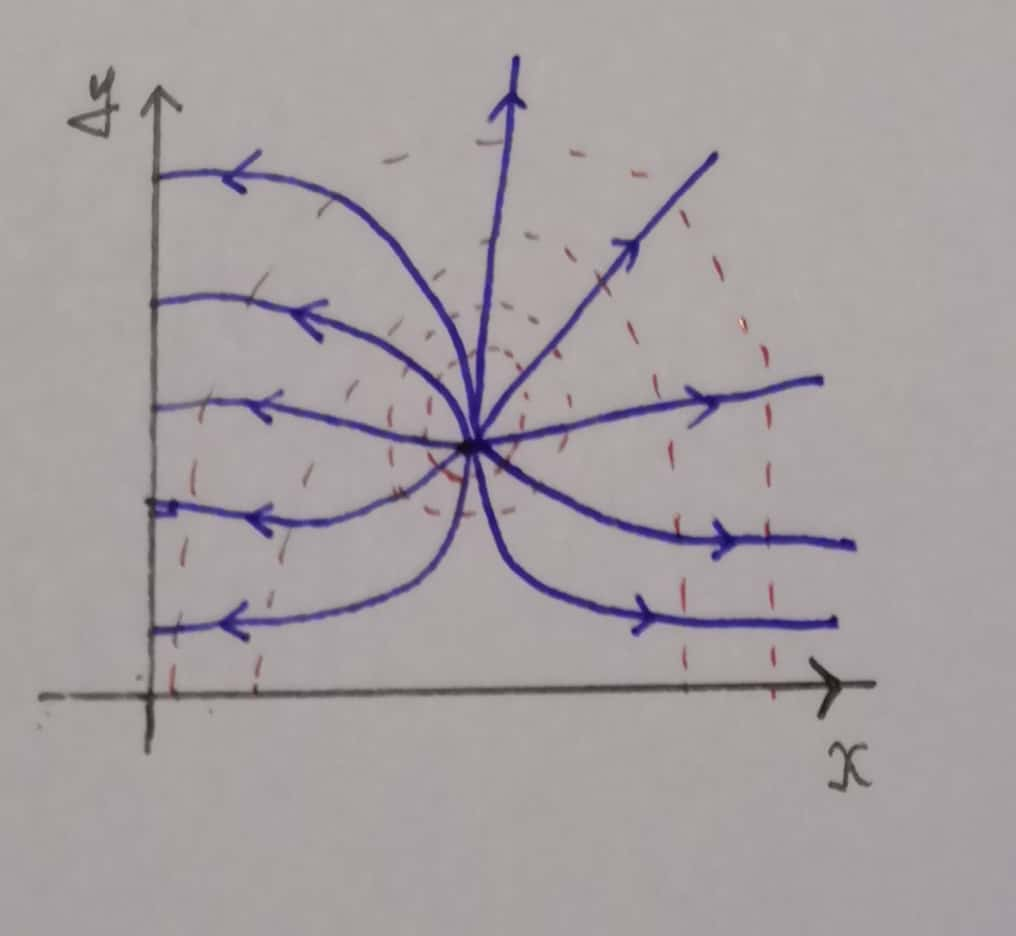
\includegraphics[width=6cm,height=4cm]{2016-6.jpg}
\end{figure}
\end{document}